\documentclass[11pt]{article}
\usepackage[textwidth=18.0cm, textheight=23.0cm, top=2.0cm]{geometry}
\usepackage{pst-all}
\usepackage{amssymb}
\usepackage{tikz}
\usepackage{underscore}\begin{document}
\pagestyle{empty}


ClassName: \underline{\textbf{Class_10.2bp-6}}
\par
BinSize: \underline{\textbf{100 × 100}}
\par
ReduceSize: \underline{\textbf{100 × 100}}
\par
TypeNum: \underline{\textbf{20}}
\par
Num: \underline{\textbf{20}}
\par
OutS: \underline{\textbf{50000}}
\par
InS: \underline{\textbf{39300}}
\par
Rate: \underline{\textbf{0.786}}
\par
UB: \underline{\textbf{5}}
\par
LB0: \underline{\textbf{5}}
\par
LB: \underline{\textbf{5}}
\par
LBWithCut: \underline{\textbf{5}}
\par
NodeCut: \underline{\textbf{0}}
\par
ExtendedNodeCnt: \underline{\textbf{1}}
\par
GenNodeCnt: \underline{\textbf{1}}
\par
PrimalNode: \underline{\textbf{0}}
\par
ColumnCount: \underline{\textbf{5}}
\par
TotalCutCount: \underline{\textbf{0}}
\par
RootCutCount: \underline{\textbf{0}}
\par
LPSolverCnt: \underline{\textbf{1}}
\par
PricingSolverCnt: \underline{\textbf{0}}
\par
BranchAndBoundNum: \underline{\textbf{1}}
\par
isOpt: \underline{\textbf{true}}
\par
TimeOnInitSolution: \underline{\textbf{600.000 s}}
\par
TimeOnPrimal: \underline{\textbf{0.000 s}}
\par
TimeOnPricing: \underline{\textbf{0.000 s}}
\par
TimeOnRmp: \underline{\textbf{0.063 s}}
\par
TotalTime: \underline{\textbf{600.307 s}}
\par
\newpage


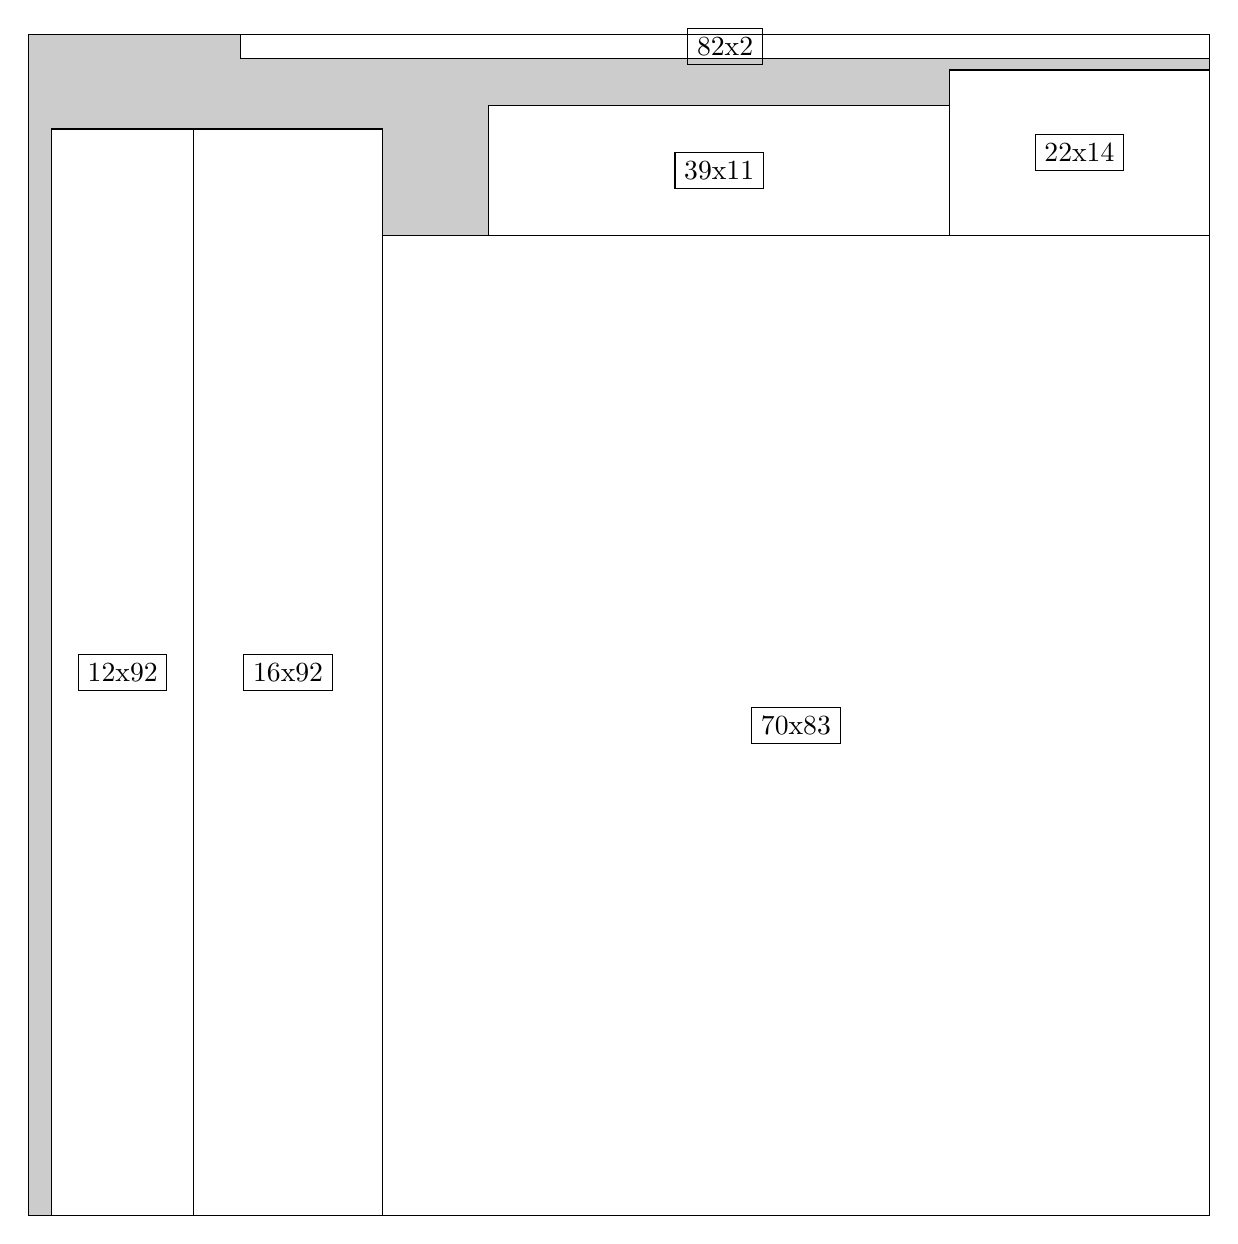
\begin{tikzpicture}[shorten >=1pt,scale=1.0,every node/.style={scale=1.0},->]
\tikzstyle{vertex}=[circle,fill=black!25,minimum size=14pt,inner sep=0pt]
\filldraw[fill=gray!40!white, draw=black] (0,0) rectangle (15.0,15.0);
\foreach \name/\x/\y/\w/\h in {70x83/4.5/0.0/10.5/12.45,22x14/11.7/12.45/3.3/2.1,39x11/5.85/12.45/5.85/1.65,16x92/2.1/0.0/2.4/13.799999999999999,12x92/0.3/0.0/1.7999999999999998/13.799999999999999,82x2/2.6999999999999997/14.7/12.299999999999999/0.3}
\filldraw[fill=white!40!white, draw=black] (\x,\y) rectangle node[draw] (\name) {\name} ++(\w,\h);
\end{tikzpicture}


w =70 , h =83 , x =30 , y =0 , v =5810
\par
w =22 , h =14 , x =78 , y =83 , v =308
\par
w =39 , h =11 , x =39 , y =83 , v =429
\par
w =16 , h =92 , x =14 , y =0 , v =1472
\par
w =12 , h =92 , x =2 , y =0 , v =1104
\par
w =82 , h =2 , x =18 , y =98 , v =164
\par
\newpage


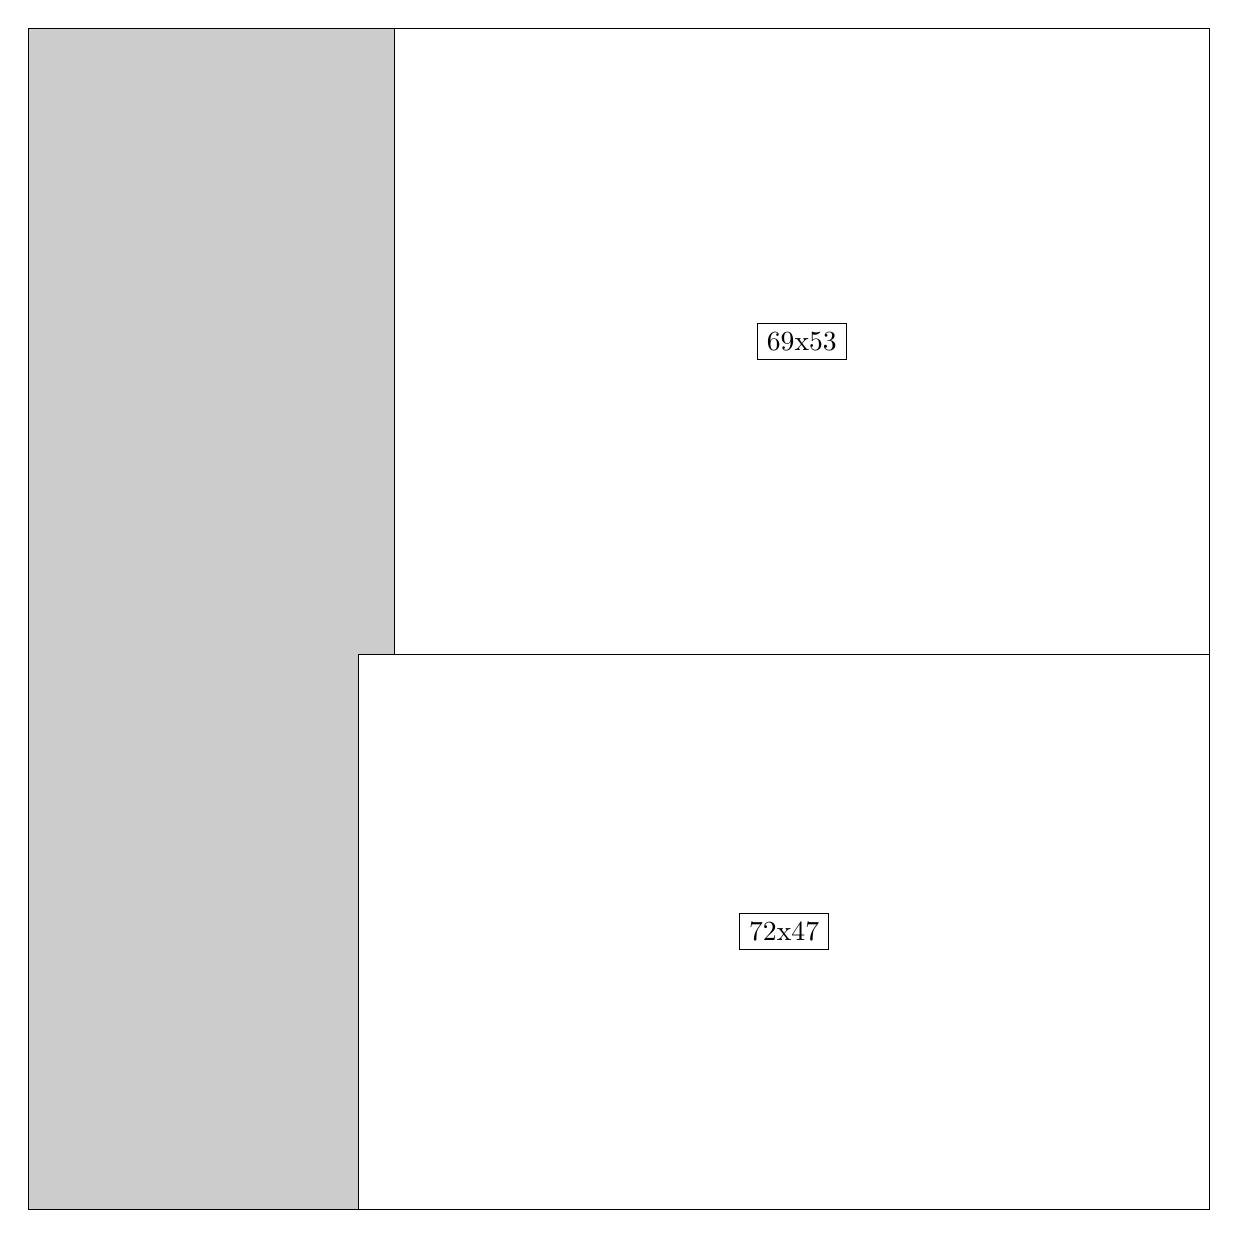
\begin{tikzpicture}[shorten >=1pt,scale=1.0,every node/.style={scale=1.0},->]
\tikzstyle{vertex}=[circle,fill=black!25,minimum size=14pt,inner sep=0pt]
\filldraw[fill=gray!40!white, draw=black] (0,0) rectangle (15.0,15.0);
\foreach \name/\x/\y/\w/\h in {72x47/4.2/0.0/10.799999999999999/7.05,69x53/4.6499999999999995/7.05/10.35/7.949999999999999}
\filldraw[fill=white!40!white, draw=black] (\x,\y) rectangle node[draw] (\name) {\name} ++(\w,\h);
\end{tikzpicture}


w =72 , h =47 , x =28 , y =0 , v =3384
\par
w =69 , h =53 , x =31 , y =47 , v =3657
\par
\newpage


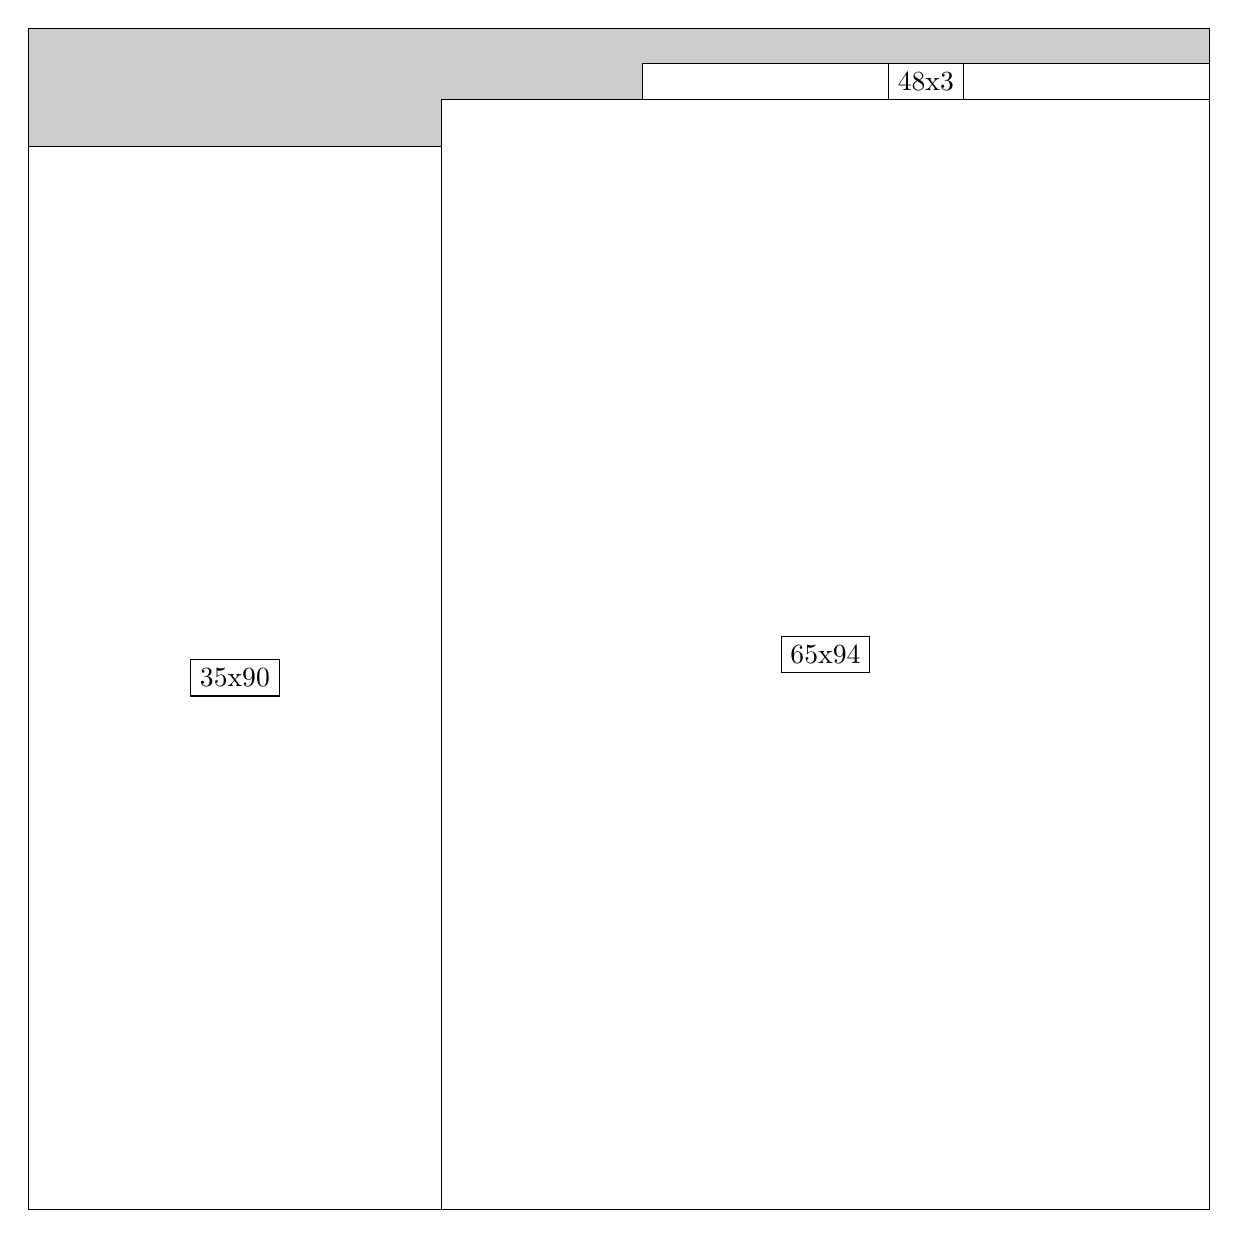
\begin{tikzpicture}[shorten >=1pt,scale=1.0,every node/.style={scale=1.0},->]
\tikzstyle{vertex}=[circle,fill=black!25,minimum size=14pt,inner sep=0pt]
\filldraw[fill=gray!40!white, draw=black] (0,0) rectangle (15.0,15.0);
\foreach \name/\x/\y/\w/\h in {65x94/5.25/0.0/9.75/14.1,48x3/7.8/14.1/7.199999999999999/0.44999999999999996,35x90/0.0/0.0/5.25/13.5}
\filldraw[fill=white!40!white, draw=black] (\x,\y) rectangle node[draw] (\name) {\name} ++(\w,\h);
\end{tikzpicture}


w =65 , h =94 , x =35 , y =0 , v =6110
\par
w =48 , h =3 , x =52 , y =94 , v =144
\par
w =35 , h =90 , x =0 , y =0 , v =3150
\par
\newpage


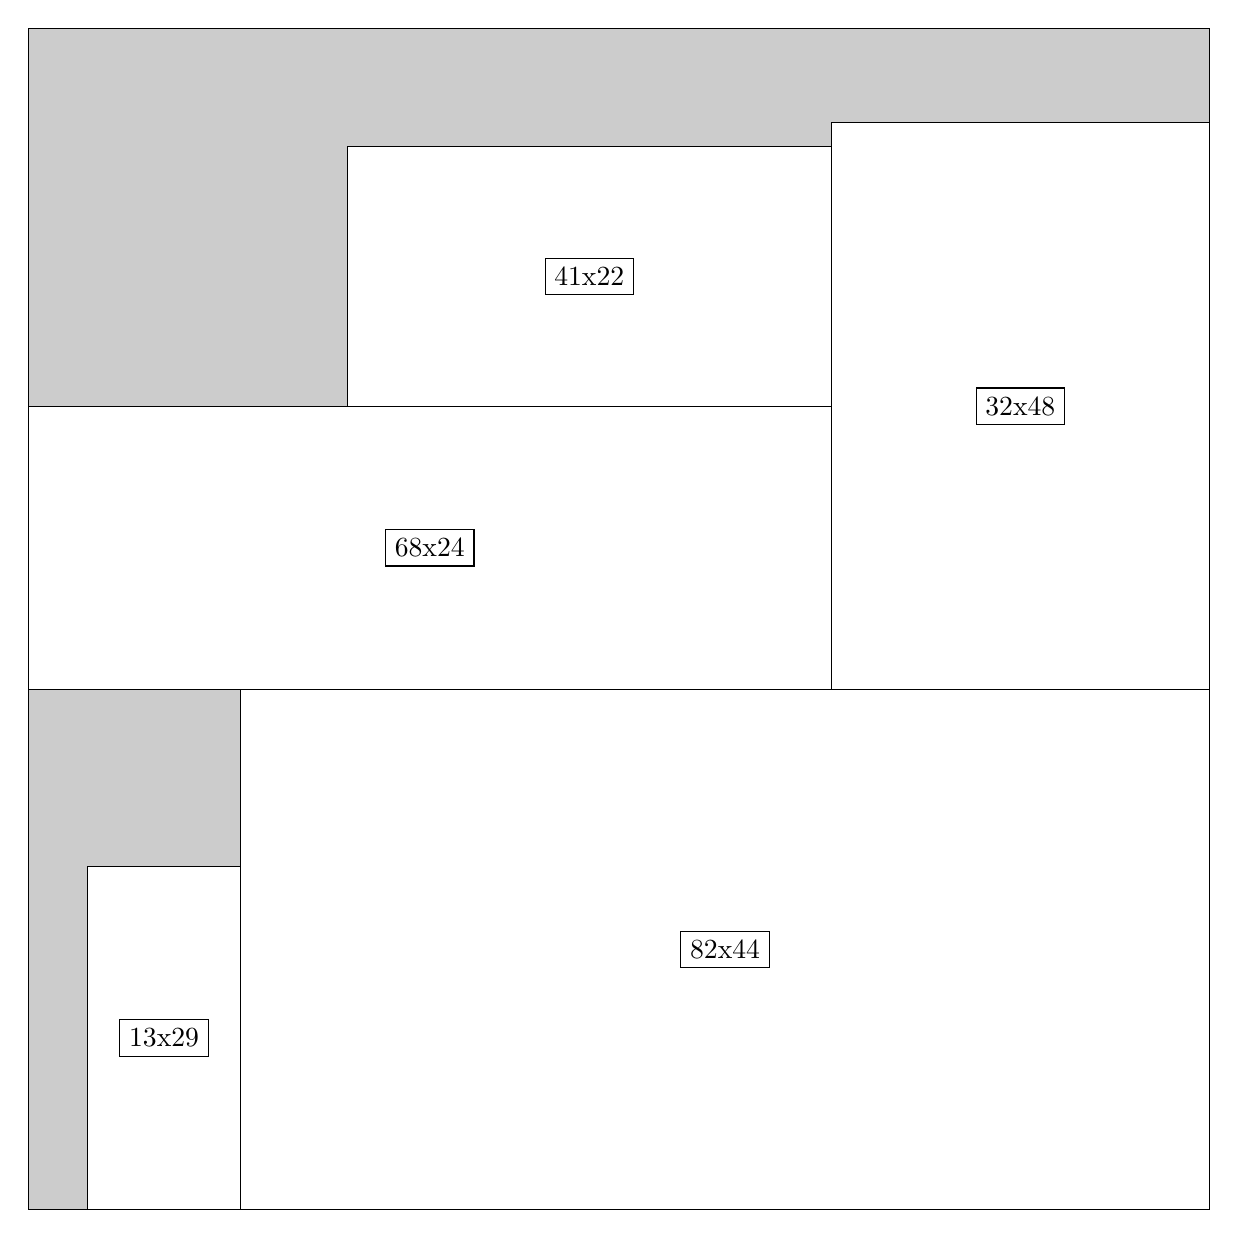
\begin{tikzpicture}[shorten >=1pt,scale=1.0,every node/.style={scale=1.0},->]
\tikzstyle{vertex}=[circle,fill=black!25,minimum size=14pt,inner sep=0pt]
\filldraw[fill=gray!40!white, draw=black] (0,0) rectangle (15.0,15.0);
\foreach \name/\x/\y/\w/\h in {82x44/2.6999999999999997/0.0/12.299999999999999/6.6,13x29/0.75/0.0/1.95/4.35,32x48/10.2/6.6/4.8/7.199999999999999,68x24/0.0/6.6/10.2/3.5999999999999996,41x22/4.05/10.2/6.1499999999999995/3.3}
\filldraw[fill=white!40!white, draw=black] (\x,\y) rectangle node[draw] (\name) {\name} ++(\w,\h);
\end{tikzpicture}


w =82 , h =44 , x =18 , y =0 , v =3608
\par
w =13 , h =29 , x =5 , y =0 , v =377
\par
w =32 , h =48 , x =68 , y =44 , v =1536
\par
w =68 , h =24 , x =0 , y =44 , v =1632
\par
w =41 , h =22 , x =27 , y =68 , v =902
\par
\newpage


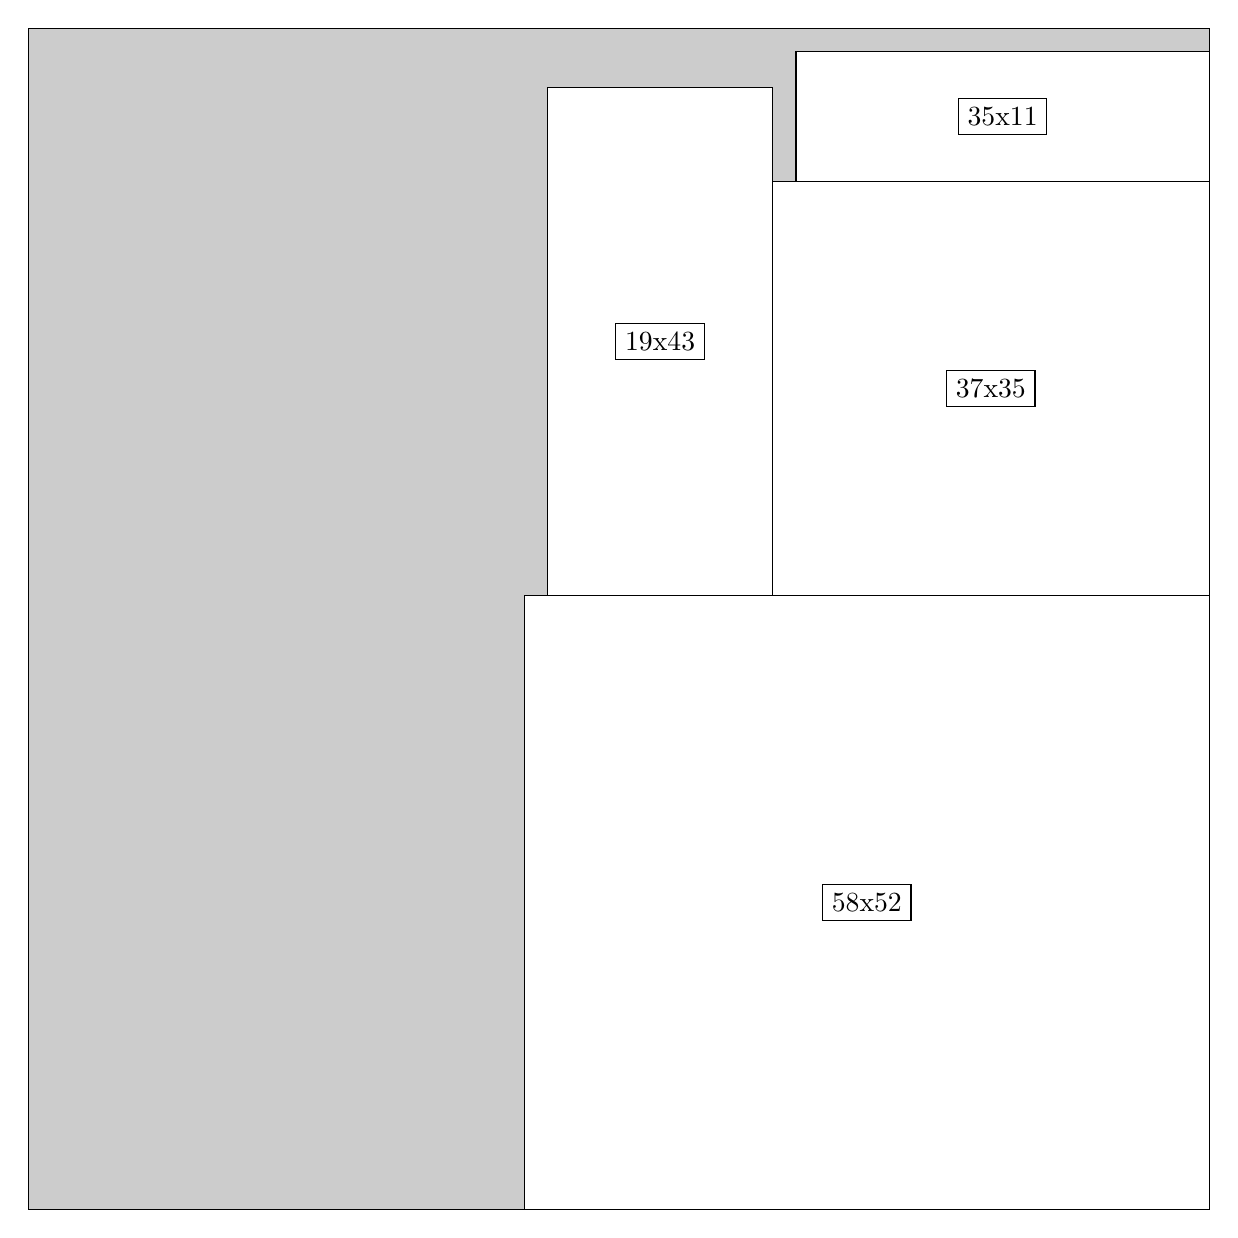
\begin{tikzpicture}[shorten >=1pt,scale=1.0,every node/.style={scale=1.0},->]
\tikzstyle{vertex}=[circle,fill=black!25,minimum size=14pt,inner sep=0pt]
\filldraw[fill=gray!40!white, draw=black] (0,0) rectangle (15.0,15.0);
\foreach \name/\x/\y/\w/\h in {58x52/6.3/0.0/8.7/7.8,37x35/9.45/7.8/5.55/5.25,35x11/9.75/13.049999999999999/5.25/1.65,19x43/6.6/7.8/2.85/6.45}
\filldraw[fill=white!40!white, draw=black] (\x,\y) rectangle node[draw] (\name) {\name} ++(\w,\h);
\end{tikzpicture}


w =58 , h =52 , x =42 , y =0 , v =3016
\par
w =37 , h =35 , x =63 , y =52 , v =1295
\par
w =35 , h =11 , x =65 , y =87 , v =385
\par
w =19 , h =43 , x =44 , y =52 , v =817
\par
\newpage


\end{document}